\documentclass[12pt,a4paper]{article}
\usepackage{tikz}
\usetikzlibrary{arrows.meta,positioning}
\usepackage{tabularx}
\usepackage{graphicx}
\usepackage{amsmath}
\usepackage{amssymb}
\usepackage{amsthm}
\usepackage{bm}
\usepackage{hyperref}
\usepackage{booktabs}
\usepackage{array}
\usepackage{geometry}
\geometry{margin=2.5cm}
\hypersetup{colorlinks=true, linkcolor=blue, citecolor=blue, urlcolor=blue}
\newtheorem{theorem}{Theorem}
\newtheorem{proposition}{Proposition}
\newtheorem{definition}{Definition}
\newtheorem{lemma}{Lemma}
\newtheorem{corollary}{Corollary}
\newtheorem{criterion}{Criterion}




\title{\textbf{Paper D-09: AI Neural Computation:\\ A Constraint-Driven Flux Dynamics (CDFD) Perspective}}
\author{Steve Bico Mujjabi, MD\\
\small Independent Researcher\\
\small Founder, Vura Labs\\
\small Kampala, Uganda\\
\small ORCID: 0009-0001-0556-5516}
\date{May 2026}


\newcommand{\EarthSuppPath}{Part\_A\_Earth\_Systems/supplementary/supplementary\_earth\_}
\newcommand{\EngSuppPath}{Part\_B\_Engineered\_Systems/supplementary/supplementary\_eng\_}
\newcommand{\SocSuppPath}{Part\_C\_Socioeconomic\_Systems/supplementary/supplementary\_soc\_}
\newcommand{\DomainSuppPath}{Part\_D\_Domain\_Applications/supplementary/supplementary\_dom\_}
\begin{document}
\maketitle

\begin{abstract}
This paper treats AI neural computation as a CDFD/AFL domain-application
hypothesis. Token flow, activation flow, gradient updates, memory retrieval,
tool calls, and inference demand are read as candidate fluxes $\Phi$ moving
through constraints $C$ such as context length, compute budget, memory bandwidth,
latency, alignment filters, and training-data structure. The goal is to define
measurable overload and recovery variables, not to claim that an AI system has
life, intention, or consciousness.
\end{abstract}

\section*{Symbol Conventions}

\noindent\textbf{CDFD/AFL Part IV symbol convention.}
\begin{center}
{\small
\begin{tabular}{p{0.15\linewidth}p{0.34\linewidth}p{0.41\linewidth}}
\hline
Symbol & Part IV meaning & Cross-domain reading \\
\hline
$\Phi$ & Driving flux or throughput & Energy, matter, signal, capital, information, traffic, force, or biological load entering a system \\
$C$ & Active constraint or capacity burden & Bottleneck, resistance, boundary, scarcity, toxicity, regulation, topology, latency, or load-bearing limit \\
$S$ & Responsiveness or adaptive surface & The system's ability to reconfigure, buffer, route, repair, learn, or preserve function under changing load \\
$M_s$ & Structural memory & Stored damage, hysteresis, inherited topology, institutional memory, trained weights, ecological legacy, or retained state \\
$\Psi_s$ & Adaptive operating ratio $(\Phi/C)\cdot S\cdot M_s$ & Local bookkeeping gauge for constrained operation, overload, recovery, or regime change; not a universal constant \\
$\Lambda$ & Life Number or capstone surplus ratio where explicitly defined & Reserved for Part II-derived life-number notation or synthesis-level surplus measures, never an undefined decoration \\
\hline
\end{tabular}
}
\end{center}

\noindent\textbf{Greek-symbol convention.}
\begin{center}
{\small
\begin{tabular}{p{0.15\linewidth}p{0.34\linewidth}p{0.41\linewidth}}
\hline
Symbol & Local role & Interpretation rule \\
\hline
$\alpha$ & Accumulation or reinforcement coefficient & Sets how fast a pathway, constraint, habit, cascade, or retained structure grows under load \\
$\beta$ & Relaxation, decay, clearance, or washout coefficient & Sets loss, recovery, damping, forgetting, degradation, or return toward baseline \\
$\gamma$ & Coupling, diffusion, redistribution, or transfer coefficient & Sets spread across nodes, layers, tissues, markets, infrastructures, media, or physical phases \\
$\delta,\epsilon$ & Perturbation, tolerance, small offset, or numerical guard & Used only as local thresholds, stability margins, measurement tolerances, or stress increments \\
$\eta,\lambda,\mu,\nu$ & Efficiency, rate, baseline, intensity, or frequency terms & Meaning is fixed by the equation, subscript, and domain-specific proxy in the paragraph where the term appears \\
$\rho,\sigma,\tau,\phi$ & Density/correlation, variability/noise, time-scale, phase, or field terms & Local coefficients only; subscripts bind them to the named pathway, domain, or experiment \\
$\Omega,\Lambda$ & Domain/state space; Life Number where defined & $\Omega$ names a modeled state space; $\Lambda$ carries life-number or synthesis notation only when the paper defines it \\
\hline
\end{tabular}
}
\end{center}

\section{Series Context}

Part I sets the flow--constraint language used here \cite{MujjabiPartI2026}.
Part II develops the Life Number and the origins-of-life use of the same notation
\cite{MujjabiPartII2026}. Part III applies AFL to biology and medicine
\cite{MujjabiPartIII2026}. This paper uses those references for notation and
series continuity, while Part IV \cite{MujjabiPartIV2026}, DOI \url{https://doi.org/10.5281/zenodo.20395901}, supplies the
cross-domain stress-test archive; it does not transfer biological claims onto AI
systems.

\section{AI Computation as Constrained Flow}

Modern AI systems move information through layered constraints. A prompt pushes
tokens into a context window; attention routes signals through a trained
parameter field; retrieval systems add external memory; inference hardware sets
latency, bandwidth, and energy limits; safety filters and tool policies add
additional routing constraints. CDFD/AFL reads the system as a flow problem with
memory: outputs depend on current demand and on structure laid down during
training, fine-tuning, caching, and retrieval.

\section{Candidate Variable Map}

\begin{table}[h]
\centering
\begin{tabularx}{\textwidth}{@{}lXX@{}}
\toprule
CDFD term & AI-system reading & Example proxy \\
\midrule
$\Phi$ & inference or update flow & token rate, request load, gradient norm \\
$C$ & active constraint & context length, memory bandwidth, latency, policy filter \\
$S$ & responsiveness & routing change, retrieval update, tool selection, scaling \\
$M_s$ & structural memory & weights, embeddings, cache, retrieval corpus, history \\
$\Psi_s$ & operating ratio & stable, saturated, brittle, or overloaded regime \\
\bottomrule
\end{tabularx}
\end{table}

\section{Failure Modes}

AI overload does not need mystical language. It can mean context saturation,
retrieval conflict, latency collapse, hallucination under sparse grounding,
memory contamination, brittle tool routing, or training-inference mismatch.
Those states are measurable only when the system boundary is clear. A local
model, a hosted model, an agent loop, and a retrieval-augmented system have
different $\Phi$, $C$, $S$, and $M_s$ proxies.

\section{Measurement Layer}

Useful measurements include token throughput, context occupancy, retrieval hit
rate, cache age, latency, refusal/error rate, grounding score, tool-call
success, memory bandwidth, gradient stability, and energy cost. A CDFD/AFL
analysis must name the failure condition before interpreting $\Psi_s$. Without
that condition, the notation only renames ordinary engineering metrics.

\section{Current Runtime Diagnostic}

The Part B adapter sweep includes an artificial-intelligence row, and the Part
E cascade diagnostic checks finite behavior and memory locking in the current
CDFD Runtime \cite{CDFDRuntime2026}. These outputs are release evidence for the
runtime, not evidence that any deployed AI system has been validated by this
paper.

\section{Tests That Can Break the Mapping}

The AI mapping weakens if the proposed variables cannot predict saturation,
latency, grounding failure, or recovery better than existing system metrics; if
$M_s$ cannot be separated from ordinary model state; or if the analysis depends
on anthropomorphic language instead of measurable system behavior.

% BEGIN PART IV MAJOR UNIVERSAL UPGRADE
\section{Major Universal Upgrade: Mechanism, Scale, and Tests}

\subsection{Observable Translation}

The paper-specific translation begins with an observable chain rather than a
verbal analogy. For AI Neural Computation, the proposed drive is training data, gradients, context, and inference requests.
The active limitation is compute, memory, data quality, architecture, bandwidth, and evaluation. Responsiveness is carried by
optimization, routing, retrieval, tool use, and oversight, while retained state is represented by
weights, optimizer state, context, fine-tuning, and deployment feedback. The outcome to explain is loss, capability, calibration, robustness, and reliability.

\begin{table}[htbp]
\centering
\small
\caption{Operational CDFD/AFL map for Paper D-09.}
\begin{tabularx}{\textwidth}{|l|X|X|}
\hline
\textbf{Term} & \textbf{Paper-specific observable meaning} & \textbf{Measurement question} \\
\hline
$\Phi$ & training data, gradients, context, and inference requests & What rate, load, gradient, or demand enters the focal system? \\
\hline
$C$ & compute, memory, data quality, architecture, bandwidth, and evaluation & Which measured bottleneck limits transfer, function, or recovery? \\
\hline
$S$ & optimization, routing, retrieval, tool use, and oversight & Which process changes effective capacity or reroutes the load? \\
\hline
$M_s$ & weights, optimizer state, context, fine-tuning, and deployment feedback & Which retained state makes equal present loads produce different futures? \\
\hline
$Y$ & loss, capability, calibration, robustness, and reliability & Which outcome is predicted out of sample, with uncertainty? \\
\hline
\end{tabularx}
\end{table}

\begin{figure}[htbp]
\centering
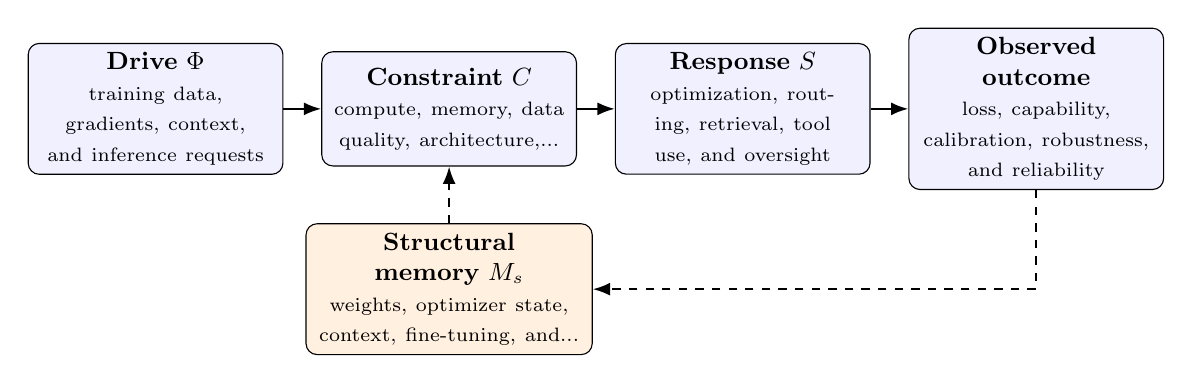
\begin{tikzpicture}[
    node distance=0.48cm,
    every node/.style={font=\small},
    box/.style={draw, rounded corners, align=center, minimum height=1.45cm, text width=3.0cm, fill=blue!6},
    memory/.style={draw, rounded corners, align=center, minimum height=1.25cm, text width=3.4cm, fill=orange!12},
    flow/.style={-{Latex[length=2.2mm]}, thick},
    feedback/.style={-{Latex[length=2.2mm]}, thick, dashed}
]
\node[box] (drive) {\textbf{Drive $\Phi$}\\\scriptsize training data, gradients, context, and inference requests};
\node[box, right=of drive] (constraint) {\textbf{Constraint $C$}\\\scriptsize compute, memory, data quality, architecture,...};
\node[box, right=of constraint] (response) {\textbf{Response $S$}\\\scriptsize optimization, routing, retrieval, tool use, and oversight};
\node[box, right=of response] (outcome) {\textbf{Observed outcome}\\\scriptsize loss, capability, calibration, robustness, and reliability};
\node[memory, below=0.72cm of constraint] (memory) {\textbf{Structural memory $M_s$}\\\scriptsize weights, optimizer state, context, fine-tuning, and...};
\draw[flow] (drive) -- (constraint);
\draw[flow] (constraint) -- (response);
\draw[flow] (response) -- (outcome);
\draw[feedback] (outcome.south) |- (memory.east);
\draw[feedback] (memory.north) -- (constraint.south);
\end{tikzpicture}
\caption{Paper D-09 observable CDFD/AFL architecture for AI Neural Computation. Solid arrows give the proposed forward chain; dashed arrows make history-dependent feedback explicit.}
\label{fig:d09-architecture}
\end{figure}

\subsection{Minimal Coupled Model}

A paper-level model must separate throughput, constraint accumulation, response,
and history. One deliberately minimal form is
\begin{align}
Y(t) &= \frac{\Phi(t)S(t)}{\epsilon + C(t)}, \\
\frac{dC}{dt} &= \alpha \Phi(t) - \beta S(t)C(t) + \gamma \mathcal{L}C(t), \\
\frac{dM_s}{dt} &= \eta C(t) - \mu M_s(t), \\
\Psi_s(t) &= \frac{\widehat{\Phi}(t)}{\epsilon+\widehat{C}(t)}\,
             \widehat{S}(t)\,[1+\omega\widehat{M_s}(t)] .
\end{align}
Here $Y$ is the measured output, $\epsilon>0$ prevents a singular denominator,
$\mathcal{L}$ is a spatial or network coupling operator, and hats denote
explicitly normalized variables. The sign and magnitude of $\omega$ must be
estimated: memory can preserve useful organization or amplify damage. No fixed
threshold is universal before the variables, normalization, and observation
scale are declared.

For this paper, the hypothesized causal sequence is specific. A change in
training data, gradients, context, and inference requests arrives faster than optimization, routing, retrieval, tool use, and oversight can compensate.
This raises or redistributes compute, memory, data quality, architecture, bandwidth, and evaluation. If the load persists,
the retained state encoded by weights, optimizer state, context, fine-tuning, and deployment feedback changes the next response, so a later event of equal
magnitude can produce a different trajectory in loss, capability, calibration, robustness, and reliability. The
scientific task is to estimate that sequence against the best ordinary model of
the domain, not merely to redescribe the outcome after it occurs.

\subsection{Cross-Scale Universality Without Mechanistic Erasure}

For the domain applications family, the universal comparison is a disciplined translation test across systems with very different material mechanisms. A valid mapping preserves the baseline science of the domain, declares the scale of every variable, and earns its place through a discriminating prediction rather than resemblance alone. \cite{Holling1973,Turing1952,Shannon1948,BakTangWiesenfeld1987}
The CDFD programme is cumulative: Part I supplies the flow--constraint
foundation \cite{MujjabiPartI2026}; Part II asks when maintained throughput
supports persistent organized states \cite{MujjabiPartII2026}; Part III
develops adaptive limitation and biological memory \cite{MujjabiPartIII2026};
and Part IV \cite{MujjabiPartIV2026} tests how much of that architecture
survives translation. The CDFD Runtime \cite{CDFDRuntime2026} supplies a
reproducible numerical stress surface, but it does not substitute for the
domain evidence named here.

The required scale declaration for this paper is nanoseconds to deployment lifetimes; parameters to AI ecosystems. At short
scales, the key question is whether the incoming drive is transmitted,
buffered, or diverted. At intermediate scales, response changes effective
capacity and network exposure. At long scales, retained structure can alter the
state space itself. A result is genuinely cross-scale only when the aggregation
rule is stated and the same conclusion is not an artifact of averaging.

\subsection{Evidence Ladder and Discriminating Tests}

\begin{table}[htbp]
\centering
\small
\caption{Evidence ladder for Paper D-09. Each rung can fail independently.}
\begin{tabularx}{\textwidth}{|p{0.17\textwidth}|X|X|}
\hline
\textbf{Test} & \textbf{Design} & \textbf{Discriminating result} \\
\hline
Proxy audit & Measure training curves, ablations, activations, evaluations, incidents, and distribution shifts and preregister how each record maps to $\Phi$, $C$, $S$, $M_s$, and $Y$. & The mapping fails if proxies are non-identifiable, circular, or change meaning across cases. \\
\hline
Load ramp & Apply or observe a capacity bottleneck or distribution shift after training while estimating the dominant constraint and response time. & A threshold claim requires a reproducible nonlinear change and uncertainty bounds, not a visually chosen breakpoint. \\
\hline
Recovery and memory & Match present load across units with different histories, then compare recovery paths. & The memory claim requires history-dependent divergence after current conditions are controlled. \\
\hline
Model comparison & Compare the baseline domain model with and without the CDFD/AFL state variables using held-out data. & The paper's stated falsifier is: CDFD variables do not improve scaling, adaptation, or failure prediction. \\
\hline
\end{tabularx}
\end{table}

The strongest practical design combines a prospective perturbation with a
recovery window. The load-ramp phase estimates where constraint begins to rise
faster than output. The recovery phase estimates $\beta$ and $\mu$, separating
fast relaxation from persistent memory. A topology or coupling intervention
then asks whether rerouting changes the cascade as predicted. Null results are
informative because they identify domains in which the universal notation adds
no measurable value.

\subsection{Research Programme and Boundary Conditions}

The immediate research programme has four steps. First, construct a documented
dataset from training curves, ablations, activations, evaluations, incidents, and distribution shifts and retain raw units before normalization.
Second, fit a baseline domain model and report its calibration and out-of-sample
error. Third, add the smallest identifiable CDFD/AFL state extension and test
whether it improves prediction of loss, capability, calibration, robustness, and reliability. Fourth, repeat the
analysis across the declared scale range and publish negative cases as part of
the universality audit.

Three boundaries are non-negotiable. Correlation between flow and failure does
not identify a constraint mechanism. A fitted memory term does not prove that
the stored state has the same material meaning in another domain. Finally, a
runtime cascade is evidence about the implementation, not evidence that the
real system follows it. The paper becomes stronger when it can say precisely
where the translation stops.


% END PART IV MAJOR UNIVERSAL UPGRADE

\section{Conclusion}

AI neural computation is a strong stress test for Part IV because it has visible
flow, constraint, responsiveness, and memory. The claim stays modest: CDFD/AFL
may help audit overload and recovery in AI systems when the variables are
measured plainly.

\section*{Conflict of Interest}
The author declares no conflict of interest.

\section*{Data Availability}
Part-specific runtime diagnostics are under each Part's \path{outputs/} directory.

Release-wide code: \path{Part_E_Synthesis/supplementary/}.

Generated summaries: \path{Part_E_Synthesis/outputs/}.

Figures: \path{Part_E_Synthesis/figures/}.


\section{Reference Layer}

\bibliographystyle{plain}
\bibliography{universal_afl_references}
\end{document}
